\documentclass[tikz]{standalone}

\begin{document}
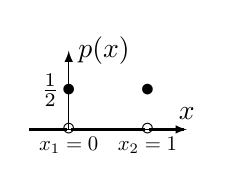
\begin{tikzpicture}
  \draw[-latex] (-0.5,0) -- (1.5,0) node[above] {\(x\)};
  \draw[-latex] (0,0)--(0,1) node[right] {\(p(x)\)};
  \node[below,scale=0.75] at (0,0) {\(x_1=0\)};
  \node[below,scale=0.75] at (1,0) {\(x_2=1\)};
  \node[left] at (0,0.5) {\(\frac{1}{2}\)};
  \node at (0,0.5) {\(\bullet\)};
  \node at (1,0.5) {\(\bullet\)};
  \node at (0,0) {\(\circ\)};
  \node at (1,0) {\(\circ\)};
  \draw[very thick] (-0.5,0) -- (-0.025,0);
  \draw[very thick] (0.025,0) -- (0.975,0);
  \draw[very thick] (1.025,0) -- (1.46,0);
\end{tikzpicture}
\end{document}
